%%%%%%%%%%%%%%%%%%%%%%%%%%%%%%%%%%%%
% Lesson Plan (50 minutes)
%%%%%%%%%%%%%%%%%%%%%%%%%%%%%%%%%%%%
\begin{frame}
    \frametitle{Lesson Plan}
    \begin{itemize}
        \item xx min Lecture: last week we did a lot of tests and inference - but how strong are our conclusions? is there a way to measure that?
        \item xx min Lecture: first, review decision errors (like slides 44-45)
        \item xx min Edfinity quiz (short): decision errors, error rates practice (review)
        \item xx min Lecture: set up a motivating example, calculate SE and minimum effect size (like slides 47-48)
        \item xx min Lecture: finally, define power
        \item xx min Edfinity quiz: what sample size will lead to a power of XX\% for this test? (like slide 50, maybe 2 such examples) 
        \item xx min Lecture: review quiz answer(s), recap procedure to computing power and how to achieve desired power (like slides 51-52)
        % TODO: maybe make the last point another quiz? i.e asking "what do you think might increase the power of this test? (open answer) 
        % then review all the factors
    \end{itemize}
\end{frame}

%%%%%%%%%%%%%%%%%%%%%%%%%%%%%%%%%%%%
% Learning objectives:
%%%%%%%%%%%%%%%%%%%%%%%%%%%%%%%%%%%%
\begin{frame}
    \frametitle{Learning Objectives}
    \begin{itemize}
        \item \textbf{M1, LO3: Use R for Data Management and Exploration:} Utilize R to load, pre-process, and explore data through visualization and summarization techniques.
        \item \textbf{M3, LO1: Understand Point Estimates and Sampling Variability:} Define a sample statistic (point estimate) for a population parameter, and explain how it varies across different samples.
        \item \textbf{M3, LO3: Calculate and Interpret Standard Error:} Calculate the standard error for proportions and interpret it as a measure of sampling variability.
        \item \textbf{M3, LO4: Explain Hypothesis Testing and Its Limitations:} Discuss the use cases and potential issues with hypothesis testing, including the interpretation of results.
        \item \textbf{M3, LO6: Distinguish Statistical vs. Practical Significance:} Differentiate between statistical significance and practical significance, and explain the implications of each.
        \item \textbf{M4, LO2: Design and Interpret Confidence Intervals:} Design, execute, and interpret confidence intervals for the population proportion.
        \item \textbf{M4, LO6: Conduct and Interpret t-Tests:} Design, execute, and interpret t-tests for a single population mean, a difference of paired means, and a difference of independent means, calculating the standard error appropriately for each. Describe how to obtain a p-value for a t-test and a critical t-score for a confidence interval.    
        \item \textbf{M4, LO7: Calculate Test Power and Evaluate Factors:} Calculate the power of a test for a given effect size and significance level, and explain how the power would change with variations in effect size, sample size, significance level, or standard error.
    \end{itemize}
\end{frame}
    
%%%%%%%%%%%%%%%%%%%%%%%%%%%%%%%%%%%%
% TODO: Copy and adapt these slides base on the lesson plan
%%%%%%%%%%%%%%%%%%%%%%%%%%%%%%%%%%%%

\section{Computing the power for a 2-sample test}

%%%%%%%%%%%%%%%%%%%%%%%%%%%%%%%%%%%%

\begin{frame}
\frametitle{}

\begin{center}
\begin{tabular}{l l | c c}
\multicolumn{2}{c}{} & \multicolumn{2}{c}{\textbf{Decision}} \\
& & fail to reject $H_0$ &  reject $H_0$ \\
  \cline{2-4}
& $H_0$ true & \onslide<4->{\green{$1 - \alpha$}} & \onslide<2->{\orange{Type 1 Error, $\alpha$}} \\
\raisebox{1.5ex}{\textbf{Truth}} & $H_A$ true &  \onslide<3->{\orange{Type 2 Error, $\beta$}} & \onslide<5->{\green{Power, $1 - \beta$}} \\
  \cline{2-4}
\end{tabular}
\end{center}

\pause

\begin{itemize}
\item Type 1 error is rejecting $H_0$ when you shouldn't have, and the probability of doing so is $\alpha$ (significance level)

\pause 

\item Type 2 error is failing to reject $H_0$ when you should have, and the probability of doing so is $\beta$ (a little more complicated to calculate)

\pause 

\item \hl{Power} of a test is the probability of correctly rejecting $H_0$, and the probability of doing so is $1 - \beta$

\pause 

\item In hypothesis testing, we want to keep $\alpha$ and $\beta$ low, but there are inherent trade-offs.

\end{itemize}

\end{frame}

%%%%%%%%%%%%%%%%%%%%%%%%%%%%%%%%%%%%

\begin{frame}
\frametitle{Type 2 error rate}

If the alternative hypothesis is actually true, what is the chance that we make a Type 2 Error, i.e. we fail to reject the null hypothesis even when we should reject it?

\begin{itemize}

\item The answer is not obvious.

\item If the true population average is very close to the null hypothesis value, it will be difficult to detect a difference (and reject $H_0$).

\item If the true population average is very different from the null hypothesis value, it will be easier to detect a difference.

\item Clearly, $\beta$ depends on the \hl{effect size} ($\delta$)
\end{itemize}

\end{frame}

%%%%%%%%%%%%%%%%%%%%%%%%%%%%%%%%%%%%

\begin{frame}
\frametitle{Example - Blood Pressure (BP), hypotheses}

{\dq
{\footnotesize
Suppose a pharmaceutical company has developed a new drug for lowering blood pressure, and they are preparing a clinical trial to test the drug's effectiveness. They recruit people who are taking a particular standard blood pressure medication, and half of the subjects are given the new drug (treatment) and the other half continue to take their current medication through generic-looking pills to ensure blinding (control). What are the hypotheses for a two-sided hypothesis test in this context?
}
}

\pause

\soln{
\begin{align*}
H_0&: \mu_{treatment} - \mu_{control} = 0 \\
H_A&: \mu_{treatment} - \mu_{control} \ne 0  
\end{align*}
}

\end{frame}

%%%%%%%%%%%%%%%%%%%%%%%%%%%%%%%%%%%%

\begin{frame}
\frametitle{Example - BP, standard error}

{\dq
{\footnotesize
Suppose researchers would like to run the clinical trial on patients with systolic blood pressures between 140 and 180 mmHg. Suppose previously published studies suggest that the standard deviation of the patients' blood pressures will be about 12 mmHg and the distribution of patient blood pressures will be approximately symmetric. If we had 100 patients per group, what would be the approximate standard error for difference in sample means of the treatment and control groups?
}
}

\pause

\soln{
\[ SE = \sqrt{ \frac{12^2}{100} + \frac{12^2}{100} } = 1.70 \]
}

\end{frame}

%%%%%%%%%%%%%%%%%%%%%%%%%%%%%%%%%%%%

\begin{frame}
\frametitle{Example - BP, minimum effect size required to reject $H_0$}

{\dq
{\footnotesize
For what values of the difference between the observed averages of blood pressure in treatment and control groups (effect size) would we reject the null hypothesis at the 5\% significance level?}
}

\pause

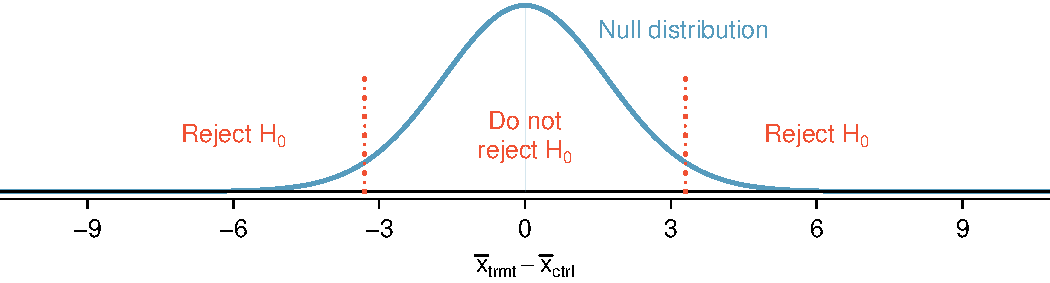
\includegraphics[width=\textwidth]{7-4_power/figures/power/power_null_B_0_1-7_with_rejection_region}

\pause

The difference should be at least 
\[ 1.96 * 1.70 = 3.332 \] 
or at most 
\[ -1.96 * 1.70 = 3.332. \]

\end{frame}

%%%%%%%%%%%%%%%%%%%%%%%%%%%%%%%%%%%%

\begin{frame}
\frametitle{Example - BP, power}

{\dq
{\footnotesize
Suppose that the company researchers care about finding any effect on blood pressure that is 3 mmHg or larger vs the standard medication. What is the power of the test that can detect this effect?
}}

\pause

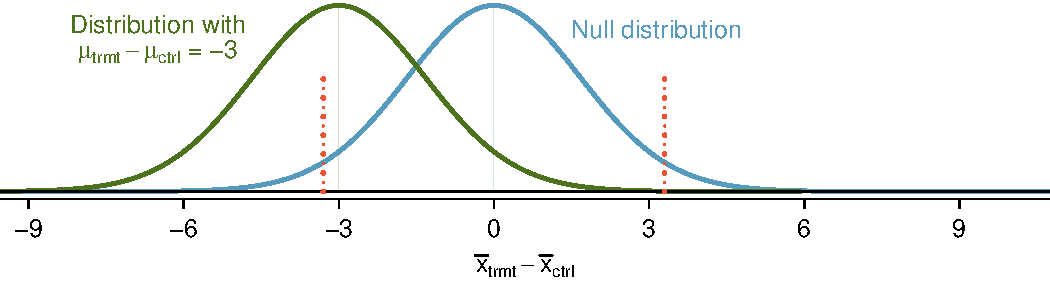
\includegraphics[width=\textwidth]{7-4_power/figures/power/power_null_C_0_1-7_with_alt_at_3}

\pause

\[ Z = \frac{-3.332 - (-3)}{1.70} = -0.20 \]

\pause

\[ P(Z < -0.20) = 0.4207 \]

\end{frame}

%%%%%%%%%%%%%%%%%%%%%%%%%%%%%%%%%%%%

\begin{frame}
\frametitle{Example - BP, required sample size for 80\% power}

{\dq
{\footnotesize
What sample size will lead to a power of 80\% for this test?
}}

\pause

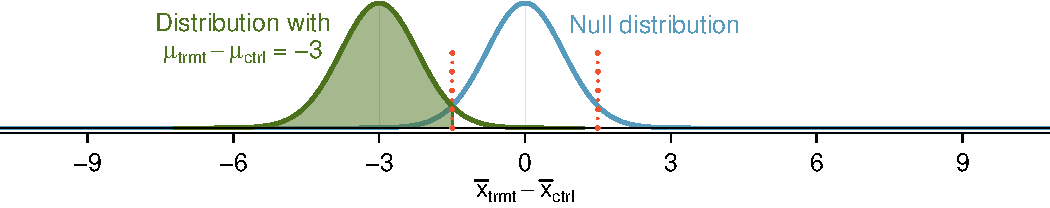
\includegraphics[width=\textwidth]{7-4_power/figures/power/power_null_0_0-76_with_alt_at_3_and_shaded}

\pause

\[ SE = \frac{3}{2.8} = 1.07142 \]

\pause

\[ 1.07142 = \sqrt{ \frac{12^2}{n} + \frac{12^2}{n} } \]

\pause

\[ n = 250.88 \rightarrow n \ge 251 \]

\end{frame}

%%%%%%%%%%%%%%%%%%%%%%%%%%%%%%%%%%%%

\begin{frame}
\frametitle{Recap}

\begin{itemize}
\item Calculate required sample size for a desired level of power
\item Calculate power for a range of sample sizes, then choose the sample size that yields the target power (usually 80\% or 90\%)
\end{itemize}
\begin{center}
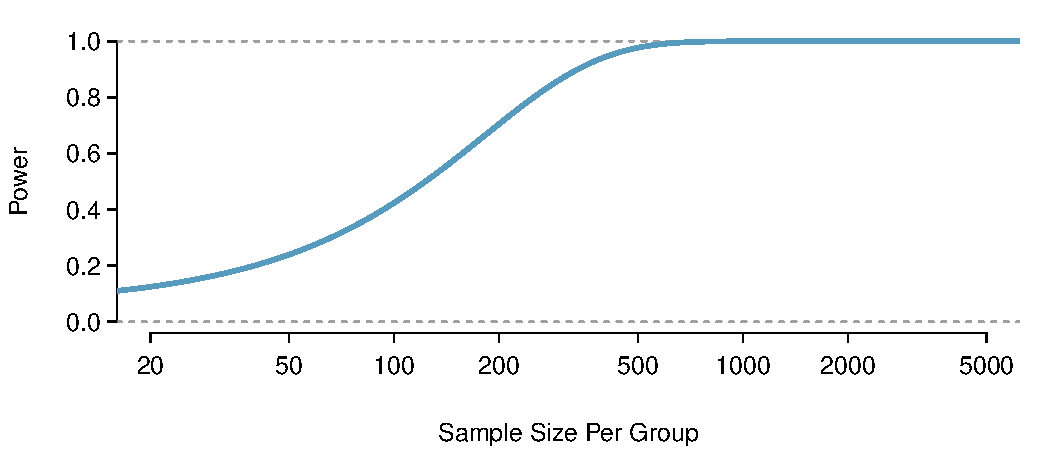
\includegraphics[width=0.7\textwidth]{7-4_power/figures/power/power_curve_neg-3}
\end{center}

\end{frame}

%%%%%%%%%%%%%%%%%%%%%%%%%%%%%%%%%%%%

\begin{frame}
\frametitle{Achieving desired power}

There are several ways to increase power (and hence decrease type 2 error rate):

\pause

{\small
\begin{enumerate}

\item Increase the sample size.

\pause

\item Decrease the standard deviation of the sample, which essentially has the same effect as increasing the sample size (it will decrease the standard error). With a smaller $s$ we have a better chance of distinguishing the null value from the observed point estimate. This is difficult to ensure but cautious measurement process and limiting the population so that it is more homogenous may help.

\pause

\item Increase $\alpha$, which will make it more likely to reject $H_0$ (but note that this has the side effect of increasing the Type 1 error rate).

\pause

\item Consider a larger effect size. If the true mean of the population is in the alternative hypothesis but close to the null value, it will be harder to detect a difference.

\end{enumerate}
}

\end{frame}

%%%%%%%%%%%%%%%%%%%%%%%%%%%%%%%%%%%%